% !TeX spellcheck = en_GB
%
\documentclass[presentation]{beamer}
\mode<presentation>{\usetheme{AMSCesenaPurpleAndGold}}
\setbeamertemplate{bibliography item}{\insertbiblabel}
%%%%%%%%%%%%%%%%%%%%%%%%%%%%%%%%%%%%%%%%%%%%%%%%%%%%%%%%%%%%%%%%%%%%%%%%%%%%%%%%
\usepackage[english]{babel}
\usepackage[utf8]{inputenc}
%
\usepackage{woa-2020-prolog-dsl-talk}
%%%%%%%%%%%%%%%%%%%%%%%%%%%%%%%%%%%%%%%%%%%%%%%%%%%%%%%%%%%%%%%%%%%%%%%%%%%%%%%%
\title[\twopkt{}: LP in Kotlin]{
    \twopkt{}: logic programming with objects \& functions in Kotlin
}
%
\author[Ciatto et al.]{
    Giovanni Ciatto$^*$
    \and
    Roberta Calegari$^\circ$
    \and
    Enrico Siboni$^\dagger$
    \\
    Enrico Denti$^\ddagger$
    \and
    Andrea Omicini$^\star$
}
%
\institute[UniBo, HES-SO]{
    $^{*\ddagger\star}$Dipartimento di Informatica -- Scienza e Ingegneria (DISI)
    \\
    $^{\circ}$Alma Mater Research Institute for Human-Centered Artificial Intelligence
    \\
    \textsc{Alma Mater Studiorum}---Università di Bologna, Italy
    \\
    \texttt{\{giovanni.ciatto, roberta.calegari, enrico.denti, andrea.omicini\}@unibo.it}
    \\\medskip
    $^\dagger$University of Applied Sciences and Arts of Western Switzerland (HES-SO)
    \\
    \texttt{enrico.siboni@hevs.ch}
}
%
\date[WOA, 2020]{
	21$^{st}$ Workshop ``From Objects to Agents'' (WOA)
	\\
	Sept. 16, 2020, Bologna, Italy
}
%%%%%%%%%%%%%%%%%%%%%%%%%%%%%%%%%%%%%%%%%%%%%%%%%%%%%%%%%%%%%%%%%%%%%%%%%%%%%%%%
\begin{document}
%%%%%%%%%%%%%%%%%%%%%%%%%%%%%%%%%%%%%%%%%%%%%%%%%%%%%%%%%%%%%%%%%%%%%%%%%%%%%%%%

%\\\\\\\\\\\\\\\\\\\\\
\frame{\titlepage}
%\\\\\\\\\\\\\\\\\\\\\

%===============================================================================
\section{Motivation \& Context}
%===============================================================================

%\\\\\\\\\\\\\\\\\\\\\
\begin{frame}[c]{Context}

	New opportunities for logic-based technologies: (X)AI and MAS

	\vfill

    \begin{block}{AI side}
        \begin{itemize}
            \item AI is shining, brighter than ever
            %
            \begin{itemize}
                \item mostly thanks to the advances in ML and sub-symbolic AI
            \end{itemize}

            \item[$\Rightarrow$] symbolic AI is gaining momentum because of eXplanable AI (XAI)
            %
            \begin{itemize}
                \item[!] hybrid solution mixing logic \& data-driven AI are flourishing \ccite{xaisurvey-ia2020}
            \end{itemize}
        \end{itemize}
    \end{block}

	\vfill

    \begin{block}{MAS side}
        The MAS community is eager for logic-based technologies \ccite{lptech4mas-jaamas2020}
        %
        \begin{itemize}
            \item to support agents' knowledge representation, reasoning, or execution

            \item or to prove MAS properties

            \item[!] despite few mature tech. exist, and even fewer are actively maintained
        \end{itemize}
    \end{block}
\end{frame}
%\\\\\\\\\\\\\\\\\\\\\

%\\\\\\\\\\\\\\\\\\\\\
\begin{frame}[c]{Motivation}

    \begin{alertblock}{The problem with logic-based technologies}
        There is technological barrier slowing
        %
        \begin{itemize}
            \item the adoption of logic programming (LP) as paradigm
            \item the exploitation of logic-based technologies
        \end{itemize}
        %
        while programming \emph{in the large}
    \end{alertblock}

    \vfill

    \begin{itemize}
        \item $\overbrace{\text{mainstream programming languages}}^\text{\itshape e.g. Scala, Kotlin, Python, C\#}$ are blending several paradigms
        %
        \begin{itemize}
            \item[e.g.] imperative, object-oriented (OOP), and functional programming (FP)
            \item except LP!
        \end{itemize}

        \vfill

        \item $\underbrace{\text{mainstream platforms}}_\text{\itshape e.g. JVM, .NET, JS, Python}$ are poorly interoperable with logic-based tech.
    \end{itemize}

\end{frame}
%\\\\\\\\\\\\\\\\\\\\\

%\\\\\\\\\\\\\\\\\\\\\
\begin{frame}{Motivating example -- SWI-Prolog's FLI for Java}

    \begin{itemize}
        \item Prolog \ccite{ColmerauerR93} implementors rely on Foreign Language Interfaces (FLI) \ccite{Bagnara2002}
        %
        \begin{itemize}
            \item (mostly targetting Java, or C)
        \end{itemize}

        \vfill

        \item For instance, SWI-Prolog comes with a FLI for Java\footnote{\url{https://jpl7.org}}:
        %
        \inputminted{java}{code/SwiFliExample.java}

        \vfill

        \item[$\rightarrow$] No paradigm harmonization between Prolog and $\underbrace{\text{the hosting language}}_\text{\itshape i.e. Java}$
    \end{itemize}

\end{frame}
%\\\\\\\\\\\\\\\\\\\\\

%\\\\\\\\\\\\\\\\\\\\\
\begin{frame}{Contribution of the paper}

\begin{itemize}
    \item Show that OOP, FP, and LP can be blended into a single language

    \vfill

    \item Propose a DSL blending Kotlin (OOP + FP) and Prolog (LP)
    \\
    \hint{DSL = domain specific language}

    \vfill

    \item Pave the way to the creation of similar DSL in mainstream languages
    %
    \begin{itemize}
    	\item[eg] Scala
    \end{itemize}
\end{itemize}

\end{frame}
%\\\\\\\\\\\\\\\\\\\\\

%===============================================================================
\section{Kotlin DSL for Prolog}
%===============================================================================

%-------------------------------------------------------------------------------
\subsection{Overview}
%-------------------------------------------------------------------------------

%\\\\\\\\\\\\\\\\\\\\\
\begin{frame}%[allowframebreaks]
\frametitle{Whet your appetite}

    Our Kotlin DSL for Prolog vs. actual Prolog

    \inputminted[fontsize=\tiny]{kotlin}{code/Relatives.kt}
    %
    \rhint{try it here: \url{https://github.com/tuProlog/prolog-dsl-example}}

\end{frame}
%\\\\\\\\\\\\\\\\\\\\\

%-------------------------------------------------------------------------------
\subsection{Principles}
%-------------------------------------------------------------------------------

%\\\\\\\\\\\\\\\\\\\\\
\begin{frame}%[allowframebreaks]
    \frametitle{Design Principles}

    \begin{block}<1>{\textbf{P\textsubscript{1}} -- The DSL \textbf{strictly extends} the hosting language}
        \begin{itemize}
            \item[$\rightarrow$] no feature of the hosting language is forbidden within the DSL
        \end{itemize}
    \end{block}

    \begin{block}<2>{\textbf{P\textsubscript{2}} -- The DSL is \textbf{interoperable} with hosting language}
        \begin{itemize}
            \item[$\rightarrow$] all features of the hosting language are allowed within the DSL
            \item[$\rightarrow$] LP is \emph{harmonised} with the hosting language paradigm(s)
        \end{itemize}
    \end{block}

    \begin{block}<3>{\textbf{P\textsubscript{3}} -- The DSL is \textbf{well encapsulated} within the hosting language}
        \begin{itemize}
            \item[$\rightarrow$] i.e. only usable within well-identifiable sections
        \end{itemize}
    \end{block}

    \begin{block}<4>{\textbf{P\textsubscript{4}} -- The DSL is \textbf{as close as possible} to Prolog}
        \begin{itemize}
            \item[$\rightarrow$] both syntactically \& semantically
        \end{itemize}
    \end{block}

\end{frame}
%\\\\\\\\\\\\\\\\\\\\\

%-------------------------------------------------------------------------------
\subsection{Functioning}
%-------------------------------------------------------------------------------

%\\\\\\\\\\\\\\\\\\\\\
\begin{frame}%[allowframebreaks]
    \frametitle{Functioning in the Kotlin case I}

    \begin{block}<1>{}
        The DSL is only enabled within \ktinline{prolog { |$\langle DSL\ block \rangle$| }} expressions
    \end{block}

    \begin{block}<2>{}
        $\begin{array}{rl}
            \text{Expressions of the form:} & \ktinline{"functor"(|$\langle e_1 \rangle$|, |$\langle e_2 \rangle$|, |$\ldots$|)}
            \\
            \text{are interpreted as terms:} & \mathtt{functor}(t_1,\ t_2,\ \ldots)
            \\\color{gray}
            \text{provided that} &\color{gray} \forall i : \langle e_i \rangle \text{ can be converted into } t_i
        \end{array}$
    \end{block}

    \begin{block}<3>{}
        Expressions of the form:
        %
        \ktinline{rule {"head"(|$\langle e_1 \rangle$|, |$\ldots$|,  |$\langle e_N \rangle$|) `if` (|$\langle e_{N+1} \rangle$| and |$\ldots$| and |$\langle e_M \rangle$|) } }
        $\begin{array}{rl}
            \text{\phantom{expre}are interpreted as rules:} & \mathtt{head}(t_1,\ \ldots,\ t_N) \impliedBy t_{N+1},\ \ldots,\ t_M
            \\\color{gray}
            \text{provided that} &\color{gray} \forall i : \langle e_i \rangle \text{ can be converted into } t_i
        \end{array}$
    \end{block}
    %
    \begin{itemize}
        \item<3> similar syntax for facts
    \end{itemize}

\end{frame}
%\\\\\\\\\\\\\\\\\\\\\

%\\\\\\\\\\\\\\\\\\\\\
\begin{frame}%[allowframebreaks]
\frametitle{Functioning in the Kotlin case II}

    \begin{block}{Within \texttt{prolog \{ $\ldots$ \} blocks}}
        \begin{itemize}
            \item \alert{\texttt{staticKb($Clause_1$, $Clause_2$, ...)}} sets up the local \alert{static} KB
            \item \alert{\texttt{dynamicKb($Clause_1$, $Clause_2$, ...)}} sets up the local \alert{dynamic} KB
            \item \alert{\texttt{solve($Query$, $Timeout$)}} returns a \emph{lazy stream} of solutions
            \item \alert{\texttt{assert($Clause$)}} appends a new clause to the local \alert{dynamic} KB
            \item $\ldots$
        \end{itemize}
    \end{block}

\end{frame}
%\\\\\\\\\\\\\\\\\\\\\

%\\\\\\\\\\\\\\\\\\\\\
\begin{frame}%[allowframebreaks]
    \frametitle{Kotlin to Prolog conversions}

    \begin{table}[]
        \centering
        \begin{tabular}{c|c}
            \textbf{Kotlin Object Type}        & \textbf{Prolog Term Type} \\
            \hline\hline
            lowercase string       & atom            \\
            uppercase string       & variable        \\
            int, long, short, byte & integer         \\
            double, float          & real            \\
            boolean                & atom            \\
            list, array, iterable  & list
        \end{tabular}
    \end{table}

\end{frame}
%\\\\\\\\\\\\\\\\\\\\\

%===============================================================================
\section{Behind the scenes}
%===============================================================================

%\\\\\\\\\\\\\\\\\\\\\
\begin{frame}%[allowframebreaks]
\frametitle{Recipe for a Prolog-like DSL}

    \begin{enumerate}
        \item A language with a flexible API
        %
        \begin{itemize}
            \item[e.g.] Kotlin, Scala, Python, Groovy, etc.
        \end{itemize}

        \vfill

        \item Full fledged API for Prolog, supporting that language
        %
        \begin{itemize}
            \item[e.g.] \twopkt{} \hint{see next slide}
        \end{itemize}

        \vfill

        \item Leverage flexibility to hide the exploitation of the API
    \end{enumerate}

\end{frame}
%\\\\\\\\\\\\\\\\\\\\\

%\\\\\\\\\\\\\\\\\\\\\
\begin{frame}%[allowframebreaks]
    \frametitle{\twopkt{} -- Overview}

    Comprehensive, modular, re-usable API covering most aspects of LP:
    %
    \begin{figure}
        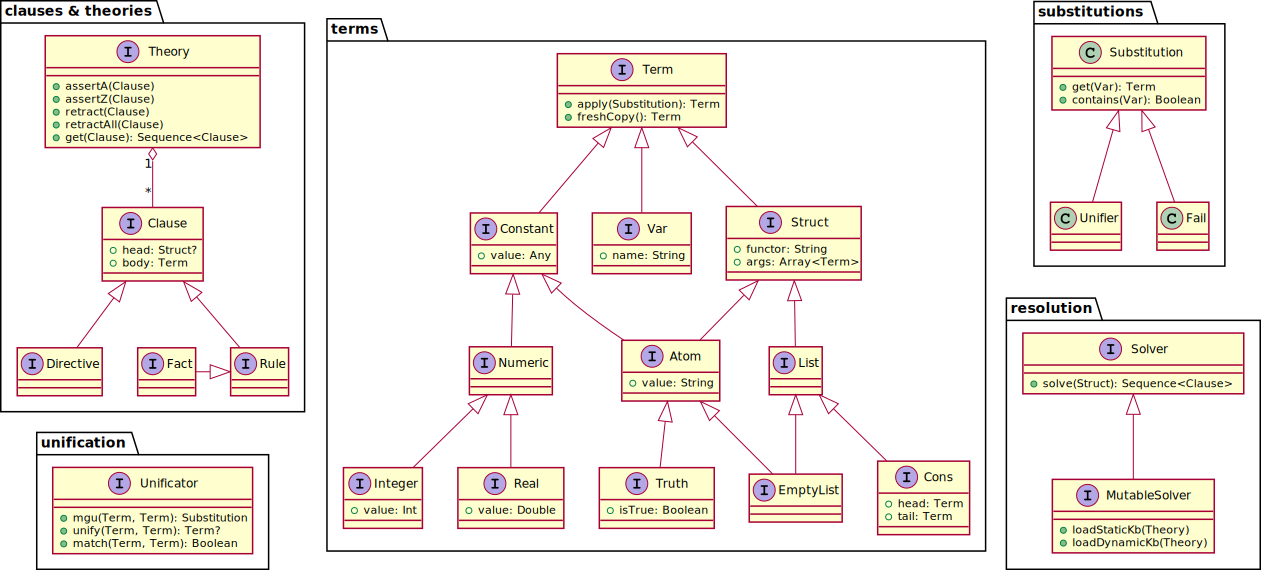
\includegraphics[width=\linewidth]{img/2p-kt-overview}
    \end{figure}
    %
    \begin{itemize}
        \item runs on several platforms (e.g., JVM, NodeJS, Browsers, Android)
        \item more info here: \url{https://github.com/tuProlog/2p-kt}
    \end{itemize}

\end{frame}
%\\\\\\\\\\\\\\\\\\\\\

%\\\\\\\\\\\\\\\\\\\\\
\begin{frame}[allowframebreaks]
    \frametitle{Kotlin mechanisms for DSL}

    We exploited 4 basic mechanisms:

    \medskip

    \begin{enumerate}
        \item Operator overloading
        %
        \inputminted{kotlin}{code/Operators.kt}

        \framebreak

        \item Block-like lambda expressions
        %
        \inputminted{kotlin}{code/Lambdas.kt}

        \item Extension methods
        %
        \inputminted{kotlin}{code/Extensions.kt}

        \framebreak

        \item Function types/lambdas with receivers
        %
        \inputminted{kotlin}{code/Receivers.kt}
    \end{enumerate}

    \framebreak

    \begin{alertblock}{This is a Kotlin-specific discussion!}
        Other languages may support DSL through different mechanisms
        %
        \begin{itemize}
            \item[e.g.] implicits in Scala
        \end{itemize}
    \end{alertblock}

\end{frame}
%\\\\\\\\\\\\\\\\\\\\\

%\\\\\\\\\\\\\\\\\\\\\
\begin{frame}%[allowframebreaks]
    \frametitle{DSL design on top of \twopkt}

    \begin{columns}
        \centering
        \begin{column}{.15\linewidth}
            \centering
            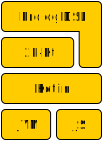
\includegraphics[width=\linewidth]{img/layers}
        \end{column}
        \hfill
        \begin{column}{.84\linewidth}
            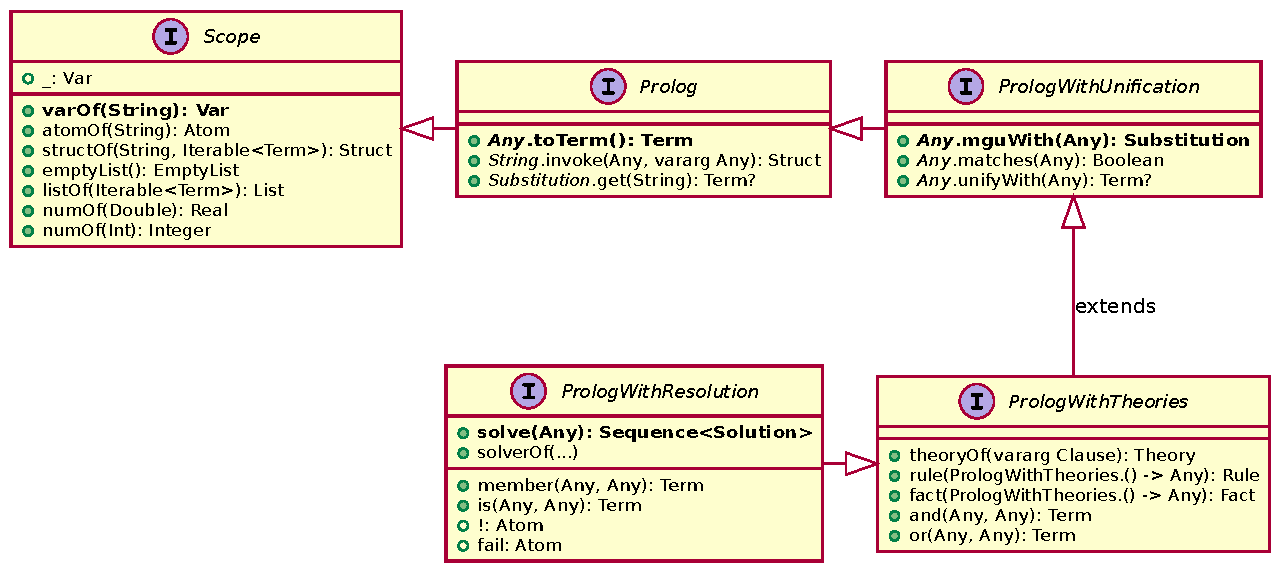
\includegraphics[width=\linewidth]{img/dsl-types}
        \end{column}
    \end{columns}

    \vfill

    \begin{itemize}
        \item Onion design with incremental features
        \item Built on top of \twopkt{} and Kotlin
    \end{itemize}

\end{frame}
%\\\\\\\\\\\\\\\\\\\\\

\section{Conclusions \& future works}

%\\\\\\\\\\\\\\\\\\\\\
\begin{frame}%[allowframebreaks]
\frametitle{Conclusions \& future works}

\begin{block}{Summing up, in this study we\ldots}
    \begin{itemize}
        \item argued LP should be integrated in modern languages/paradigms
        \item designed an in-language, DSL-based solution
        \item prototyped an actual Kotlin-based DSL for Prolog
    \end{itemize}
\end{block}

\begin{exampleblock}{In the future, we will try to\ldots}
    \begin{itemize}
        \item design Prolog-like DSL for other languages (e.g. Scala)
        \item design an agent-oriented (possibly BDI?) DSL
        \item extend \twopkt{} to support other sorts of inference mechanisms
        \item design a logic-based API for sub-symbolic AI
    \end{itemize}
\end{exampleblock}

\end{frame}
%\\\\\\\\\\\\\\\\\\\\\

%===============================================================================
\section*{}
%===============================================================================
\frame{\titlepage}

%===============================================================================
\section*{\bibname}
%===============================================================================

\setbeamertemplate{page number in head/foot}{}
%\\\\\\\\\\\\\\\\\\\\\
\begin{frame}[t,allowframebreaks,noframenumbering]\frametitle{\refname}
% \begin{frame}[c]\frametitle{\refname}
	\footnotesize
%	\scriptsize
    \bibliographystyle{plain}
	\bibliography{woa-2020-prolog-dsl-talk}
\end{frame}
%\\\\\\\\\\\\\\\\\\\\\

%%%%%%%%%%%%%%%%%%%%%%%%%%%%%%%%%%%%%%%%%%%%%%%%%%%%%%%%%%%%%%%%%%%%%%%%%%%%%%%%
\end{document}
%%%%%%%%%%%%%%%%%%%%%%%%%%%%%%%%%%%%%%%%%%%%%%%%%%%%%%%%%%%%%%%%%%%%%%%%%%%%%%%%
